\comment{AB: This is the most important section in the paper, because it contains the
main results of the paper, i.e., the constraints on QNMs using real data. It needs to
be expanded and results would need to be highlighted much better than in the current version.
I would like to suggest that besides the Table and the figure with the 2D- and 1D-posteriors
that you made (which can be contrasted with Fig. 14 of the TGR GWTC-2 paper), we could have
a new figure that is either a combination of Figs. 5 and 6 or only Fig. 5 of the
TGR GWTC-2, but for the 22 QNM frequencies for the different GW events.
Figures can be used in talks, and can capture the information much better
than a list of numbers in a Table.}

The LIGO-Virgo Collaboration recently released their testing GR
catalogue containing results \sout{of this test} for all events observed
during O3a~\cite{Abbott:2020jks}, which passed a threshold for the
total (source-frame) mass $\geq 50 \Mo$ and SNRs in the pre- and
post-merger regions $\geq 8$.The pre- and post-merger regions of the
signal are identified \sout{as} \ab{from} the \ab{signal's} power \sout{in the frequency content of the
signal} before and after the signal reaches \ab{the} peak\ab{'s}
amplitude, \sout{as} \ab{which is} determined by the maximum \ab{of the}
likelihood \ab{function}  \ab{from the} parameter-estimation \ab{analysis} \sout{template}.
\comment{AB: What does it mean ``for the purpose of Ref.''? We are using present tense in the
entire paper, except perhaps the Conclusions section.}
For the purpose of Ref.~\cite{Abbott:2020jks}, we use\sout{d} a mass
threshold and restrict\sout{ed} ourselves to the highest-mass events which
\sout{were} \ab{are} expected to be most promising to study merger-ringdown. However,
since our method relies on doing a parameter estimation on the entire
inspiral-merger-ringdown signal, we require the SNR to be beyond a
certain threshold throughout the signal for reliable parameter
estimation of the initial and final quantities. \comment{AB: there are not ``initial'' and ``final'' parameters,
there are the component masses of the holes in the binary, and the
mass of the remnant formed after merger.} In fact the SNR
threshold alone should be sufficient for the analysis, and for this
paper we have relaxed the mass threshold. This has added two events,
GW190630$\_$185205 and GW190828$\_$063405, to the list of GW events
considered in \cite{Abbott:2020jks} \abhi{Runs ongoing and looking
  promising}. Fig.~\ref{fig:o1o2_events} shows results from these two
events along with GW190519$\_$153544, GW190521$\_$074359,
GW190910$\_$112807. \comment{AB: Please improve the above paragraph
and make it clearer which choice is made for the SNR threshold and
masses, and why.}

Furthermore, for the first time, in this paper, we apply our method to
measure the QNMs to the relevant
GW events from LIGO-Virgo's O1 and O2 runs, alongside
the above events. Applying the same thresholds as above, we find three
additional events that could be included in the analysis: GW150914,
GW170104, GW170729. The other high-mass events from O1-O2, GW170809,
GW170814, GW170818 and GW170823 do not have an SNR of $8$ in the
merger-ringdown signal. For the three relevant signals, GW150914,
GW170104 and GW170729, we show the posterior distributions in
$(\df{220}, \dtau{220})$ in Fig.~\ref{fig:o1o2_events}. We also reconstruct the QNM parameters, $(\fngr{220}, \taungr{220})$
which are tabulated in Table~\ref{tab:qnm_o1o2_results} \footnote{See
  Table IV of Ref.~\cite{Abbott:2020jks} for a list of the SNR
  thresholds. The paper quotes them for the purpose of the IMR
  consistency test, but the same thresholds have been used for the
  $\pSEOB$ test, as well.} Among all the GW signals detected so far,
GW150914 (solid curve in Fig.~\ref{fig:o1o2_events}) is unique in its
loudness, leading to the first, and to date, best attempt in measuring the QNM frequencies~\cite{LSC_2016grtests,Brito:2018rfr,Carullo:2019flw,Isi:2019aib}.

%%%%%%%%%%%%%%%%%%%%%%%%%%%%%%%%%%%%%%%%%%%%%%%%%%%%%%%%%%%%%%%
% O1-O2 events
%%%%%%%%%%%%%%%%%%%%%%%%%%%%%%%%%%%%%%%%%%%%%%%%%%%%%%%%%%%%%%%
\begin{figure*}
        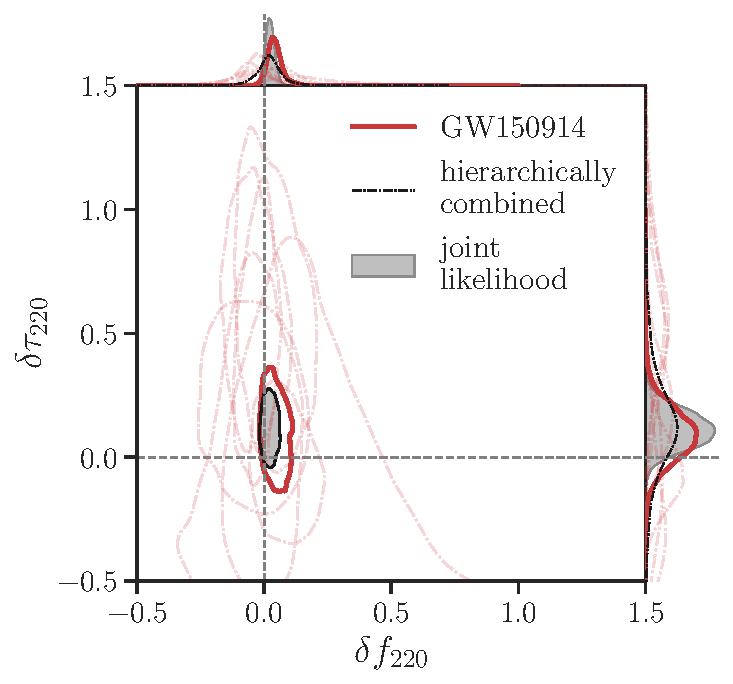
\includegraphics[width=0.5\textwidth]{figures/rin_pseob_results_v2.pdf}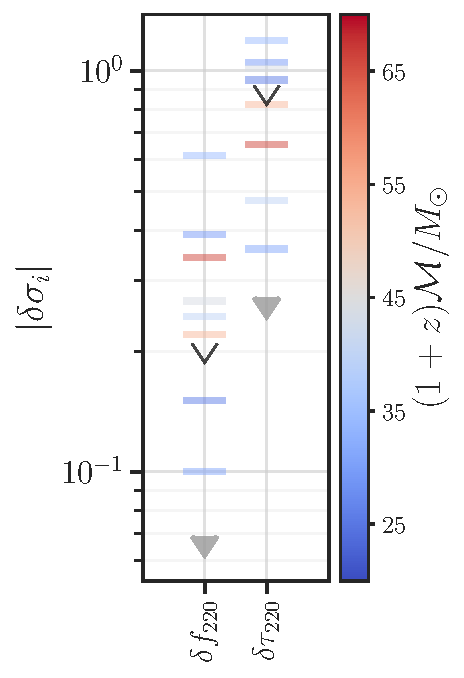
\includegraphics[width=0.3\textwidth]{figures/rin_all_events_bounds.pdf}
        \caption{\emph{Top panel}: The 90\% credible levels of the posterior probability distribution of the fractional deviations in the frequency and damping time of the $(2,\pm 2)$ QNM, $(\df{220},\dtau{220})$ and their corresponding one-dimensional marginalized posterior distributions, for events from O1, O2 and O3a passing a SNR threshold of $8$ in both the pre- and post-merger signal. The solid red curve marks the best single-event constraint, GW150914, whereas the contraints from the other events are indicated by the dash-dot curves. The joint constraints on $(\df{220},\dtau{220})$ obtained multiplying the likelihoods from individual events is given by the filled grey contours, while the hierarchical method of combination yields the black dot dashed curves. \emph{Bottom panel}: 90\% credible interval on the one-dimensional marginalised posteriors on $\delta \sigma_i=(\df{220},\dtau{220})$, colored by the median redshifted chirp mass $(1 + z)M$, inferred assuming GR. Filled gray (unfilled black) triangles mark the constraints obtained when all the events are combined by multiplying likelihoods (hierarchically).}
        \label{fig:o1o2_events}
\end{figure*}
%%%%%%%%%%%%%%%%%%%%%%%%%%%%%%%%%%%%%%%%%%%%%%%%%%%%%%%%%%%%%%%
%%%%%%%%%%%%%%%%%%%%%%%%%%%%%%%%%%%%%%%%%%%%%%%%%%%%%%%%%%%%%%%

Finally, if we assume that the fractional deviations $(\df{220},
\dtau{220})$ take the same values in multiple events, we can assume
the posterior of one event to be the prior for the next, and obtain a
joint posterior probability distribution. For $N$ observations, where
$P_j(\df{220}, \dtau{220} | d_j)$ is the posterior for the $j$-th
observation corresponding to the data set $d_j$, $j=1,\dots,N$, the joint
posterior is given by:
%
\begin{equation}
P(\df{220}, \dtau{220} | \{d_j\}) = P(\df{220}, \dtau{220}) \prod _{j=1}^N \frac{P(\df{220}, \dtau{220} | d_j) }{P(\df{220}, \dtau{220})}
\end{equation}
%
where $P(\df{220}, \dtau{220})$ is the prior on $(\df{220},
\dtau{220})$. However, since we assume the prior on $(\df{220},
\dtau{220})$ to be flat (or uniform), the joint posterior is equal to
the joint likelihood.

We show these joint likelihoods on $(\df{220}, \dtau{220})$, as well as, the corresponding \ab{1D} marginalized distributions as filled grey curves in Fig.~\ref{fig:o1o2_events}.
These are the strongest constraints on possible deviations in the measurement of $(\df{220}, \dtau{220})$ to date using our method.\comment{AG: add text on the hierarchical analysis
if we want to include that analysis. AB: we want to include that analysis.}

\comment{AB: Please write in the text (equations) the results for $(\df{220}, \dtau{220})$ for GW150914, the joint likelihood and the
hierarchically combined methods.}

%%%%%%%%%%%%%%%%%%%%%%%%%%%%%%%%%%%%%%%%%%%%%%%%%%%%%%%%%%%%%%%
% Table for LVC values
%%%%%%%%%%%%%%%%%%%%%%%%%%%%%%%%%%%%%%%%%%%%%%%%%%%%%%%%%%%%%%%
\begin{table}

\begin{tabular}{lllll}
\toprule
Event & $\fngr{220}$ (Hz) & $\taungr{220}$ (ms) & $M_f/\Mo$ & $a_f$ \\[0.075cm]
\midrule
\hline

GW150914 &
$258^{+17}_{-13}$ &
$4.5^{+1.1}_{-0.9}$ &
$71^{+9}_{-10}$ &
$0.8^{+0.1}_{-0.2}$
\\[0.075cm]

GW170104 &
$291^{+15}_{-30}$ &
$5.5^{+3.5}_{-2.4}$ &
$74^{+11}_{-20}$ &
$0.9^{+0.1}_{-0.4}$
\\[0.075cm]

GW170729 &
$152^{+13}_{-9}$ &
$10.7^{+4.2}_{-3.7}$ &
$141^{+20}_{-29}$ &
$0.9^{+0.1}_{-0.2}$
\\[0.075cm]

GW190519\_153544 &
$124^{+12}_{-13}$ &
$10.3^{+3.6}_{-3.1}$ &
$155^{+24}_{-30}$ &
$0.8^{+0.1}_{-0.3}$
\\[0.075cm]

GW190521\_074359 &
$205^{+15}_{-12}$ &
$5.3^{+1.5}_{-1.2}$ &
$86^{+12}_{-14}$ &
$0.7^{+0.1}_{-0.3}$
\\[0.075cm]

GW190630\_185205 &
$248^{+32}_{-53}$ &
$3.9^{+2.4}_{-1.8}$ &
$66^{+19}_{-42}$ &
$0.6^{+0.3}_{-0.6}$
\\[0.075cm]

GW190828\_063405 &
$258^{+201}_{-28}$ &
$4.2^{+4.2}_{-1.9}$ &
$67^{+26}_{-30}$ &
$0.8^{+0.2}_{-0.7}$
\\[0.075cm]

GW190910\_112807 &
$174^{+12}_{-8}$ &
$9.5^{+3.1}_{-2.7}$ &
$123^{+15}_{-18}$ &
$0.9^{+0.0}_{-0.1}$
\\[0.075cm]

\bottomrule
\end{tabular}
\caption{\textcolor{red}{NOT COMPLETE} \comment{AB: We would need to give also the final mass and spins. I would suggest that we list in the Table
also the results from the TGR GWTC-2 paper, obtained with our method, so that all the results are in one Table.}}
\label{tab:qnm_o1o2_results}
\end{table}

%%%%%%%%%%%%%%%%%%%%%%%%%%%%%%%%%%%%%%%%%%%%%%%%%%%%%%%%%%%%%%%
%%%%%%%%%%%%%%%%%%%%%%%%%%%%%%%%%%%%%%%%%%%%%%%%%%%%%%%%%%%%%%%
